\section{Approach Overview}
\label{sec:overview}

The goal is to infer for all memory objects of the parallelized loop high-level
properties that require minimal bookkeeping and access checks.

\begin{figure}[htp]
  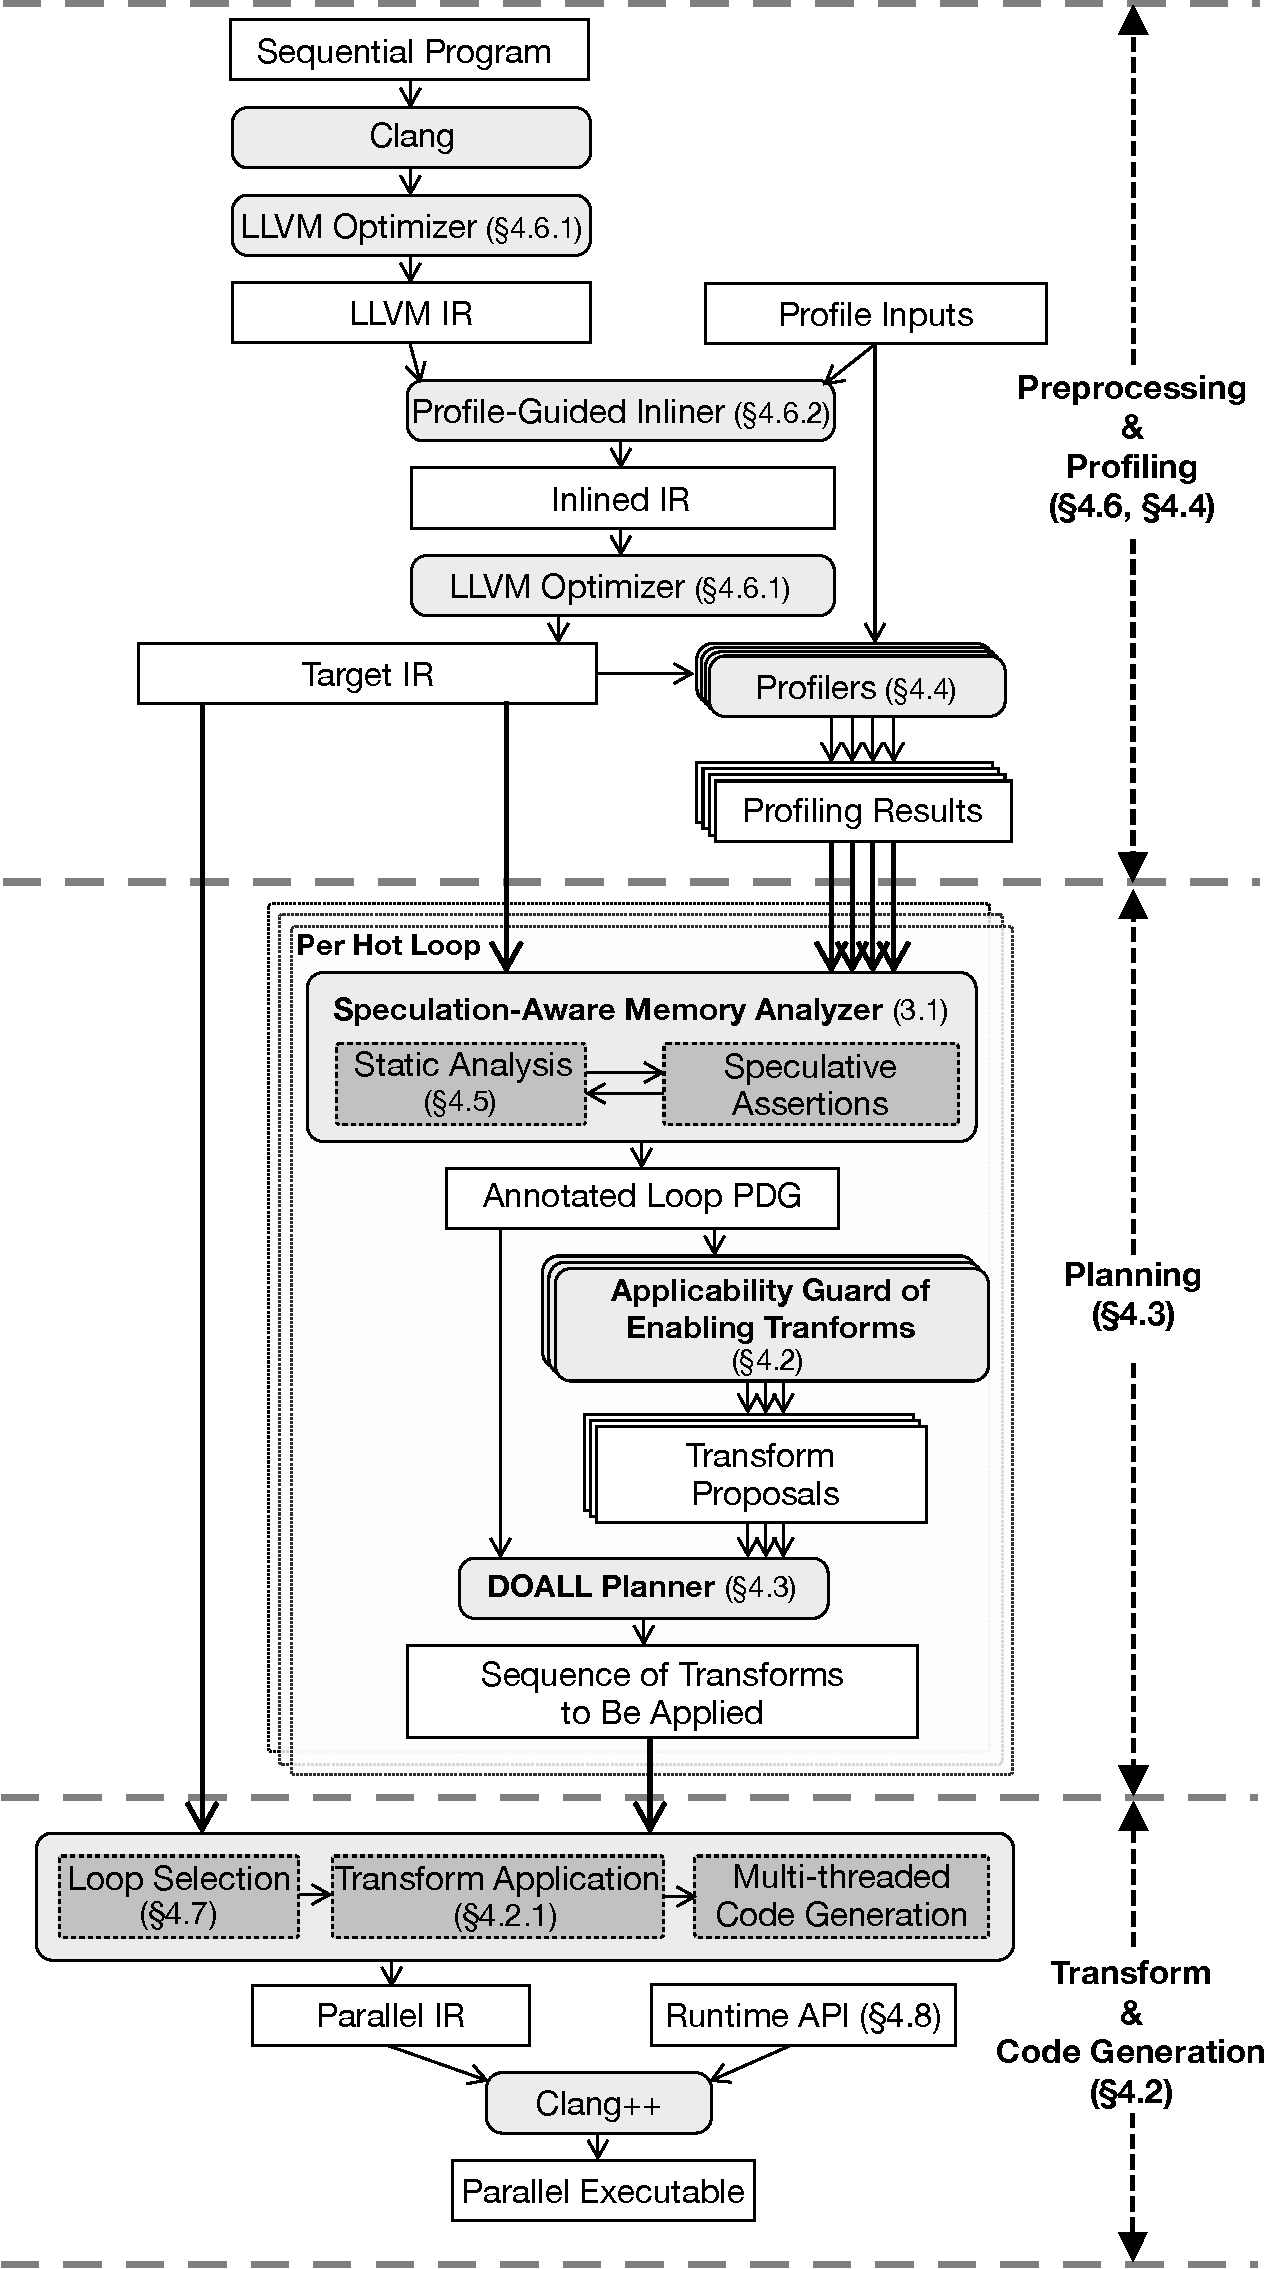
\includegraphics[width=\columnwidth]{figures/compiler-pipeline-crop}
  \caption{Compiler Pipeline Overview}
  \label{fig:compiler-pipeline}
\end{figure}

%\subsection{Memory Object Properties}
\subsection{What Memory Object Properties?}

DOALL parallelization is applicable when the loop's memory objects belong to one
of these categories: (i) private~\cite{privateer,LRPD,ARRAY_privatization} (does
not partake in any loop-carried memory flow); (ii) read-only; (iii)
local~\cite{corD,privateer,clusterDoall} (allocated and de-allocated within the
same iteration); and (iv) reduction~\cite{privateer,LRPD} (participates in a
reduction operation only).
%

To enable more efficient parallelization, we express more properties for private
memory objects. Private objects could additionally (a) be
independent~\cite{ARRAY_privatization} (no loop-carried false dependences); (b)
have loop-invariant condition for last update within the
loop~\cite{ARRAY_privatization}; (c) have predictable live-out content (not
found in prior work); or (d) not be live-out (no accesses after loop execution).
%
%Private properties (a), (b) have been explored before in the context of static
%parallelization~\cite{ARRAY_privatization}, but never before in speculative
%parallelization systems (maybe in LRPD). No prior work leveraged property (c).
%
Table~\ref{tab:priv_types} summarizes how these properties can facilitate more
efficient parallelization compared to just inferring that a memory object is
private. In short, inference of any of these four private properties allows
complete elimination of bookkeeping and access checks. Prior software
speculative systems with extended support of privatization (Privateer~\cite{},
ClusterDoall~\cite{}) are only able to infer the simple private property and
thus always require costly checks or monitoring.

\centering
\tiny
\begin{tabular}{|c|c|c|c|c|c|c|c|c|}
  \hline
  Type of Private &
  Overlap         &
  Spec Privatization &
  Other Spec Allowed    &
  Loads Checks  &
  Store Checks    &
  Last-Write Detection &
  CoW Mapping &
  Copy-out to Main \\

%%%%%%%%%%%%%%%%%%% Shared %%%%%%%%%%%%%%%%%%%%%%%%%%
 \hline
 Shared & No & - & - & - & - & - & - & - \\
 \hline
%%%%%%%%%%%%%%%%%%% Local %%%%%%%%%%%%%%%%%%%%%%%%%%
 Local Private & Any & - & $\checkmark$ & - & - & - & $\checkmark$ & - \\
 \hline
%%%%%%%%%%%%%%%%%%% Overwrite %%%%%%%%%%%%%%%%%%%%%%%%%%
 Kill Private & Complete & - & $\checkmark$ & - & - & - & $\checkmark$ &
$\checkmark$ \\
 \hline
%%%%%%%%%%%%%%%%%%% Conservative Private %%%%%%%%%%%%%%%%%%%%%%%%%%
 Static Private & No/Partial & - & $\checkmark$ & - & - &
 $\checkmark$ & $\checkmark$ & $\checkmark$ \\
 \hline
%%%%%%%%%%%%%%%%%%% Specpriv Private %%%%%%%%%%%%%%%%%%%%%%%%%%
 Privateer Private & Any & $\checkmark$ & $\checkmark$ & $\checkmark$ & $\checkmark$ &
 $\checkmark$ & $\checkmark$ & $\checkmark$ \\
 \hline
\end{tabular}




%\paragraph{Example:}
%Consider the code in figure~\ref{dijkstra_all} (taken from MiBench~\cite{} benchmark
%dijkstra, used in the evaluation of Privateer~\cite{}).
%TODO: describe the properties of all the loop memory objects in the example.


\subsection{How to Infer Memory Object Properties \\ Without Expensive Runtime
Costs?}
%\subsection{Efficient Inference of Memory Object Properties}

Characterizing the behavior of a memory object requires (i) identification of
accesses to this object within the loop and (ii) analysis of the dependences
that these accesses introduce.  This work attempts to satisfy these two
requirements by using a combination of cheap-to-validate speculative assumptions
and static analysis. For almost all the memory objects of the evaluated
benchmarks, this combination was sufficient and no use of memory speculation was
required.

\paragraph{Determine accesses of memory objects:} This task is very challenging
for general-purpose programs with pointers, dynamic allocation,and type casts.
%
%Briefly, this task entails ...
Challenges include points-to mapping from pointers to memory objects, different
objects created by the same static instruction, and presence of ``disguised''
pointers~\cite{citation3_from_privateer}.
%(not all pointer values are necessarily visible in the IR).
%
Johnson et al. ~\cite{johnson:pldi:12} recognized these challenges and proposed
an inexpensive speculative technique called separation speculation to bypass
them.
%
Using a points-to profiler, all the memory accesses are mapped to memory
objects.
%
To enable cheap validation, instead of checking at runtime that each individual
memory access points to the correct set of objects, it groups memory objects,
based on their access pattern, to a few heaps and just ensures separation of
these heaps at runtime.
%

TODO: explain more why this check is sufficient (if all objects share the same
properties then points-to family validation is enough. The example will make
this clear but maybe it needs to be clarified here)

%
%Similarly, to Privateer~\cite{johnson:pldi:12}, this work groups memory objects
%to families with objects that share the same set of properties.  Inexpensive
%checks with neither bookkeeping nor inter-worker communication ensure that all
%accesses point to the correct heap. Namely, it validates that that the profiled
%points-to information are accurate on a points-to family level.
%
Note that in Privateer's monolithic design separation speculation is entangled
with memory speculation resulting in high runtime overheads (see
section~\ref{eval}).
%
This work instead employs a modular design where separation speculation is
decoupled from other speculative techniques and can be used in conjunction with
other speculation or analysis to infer memory object properties.

%In contrast with Privateer, we decouple separation speculation from the
%classification of objects to families. Privateer's monolithic design forces
%usage of separation speculation along with memory speculation resulting in
%increased runtime overhead (see section~\ref{eval}).
%%
%This work instead uses a modular design where separation speculation in
%conjuction with other inexpensive speculation and static analysis infer and
%validate memory object properties.


\paragraph{Dependence Analysis:}

TODO: describe speculative techniques and analysis used to analyze the
dependences of memory access.  One dependence characterization might require
collaboration of different passes.

analysis of the dependences
that these accesses introduce.

%In the past, privateer monolithically combined separation logic with
%mem spec to infer properties.
%no usage of static analusos/

%Mention the two speculative ones
%plus the usage of separation logic
%and the rest are the analysis algorithms from CAF


%First, a quick description of the used static and speculative analyses in our
%example:
%%
%\begin{itemize}
%%
%\item \textit{Static Analysis} (see ~\cite{johnson:17:cgo} for more information)
%%
%  \begin{itemize}
%%
%  \item \textit{Alias Analysis}: an ensemble of analysis algorithms that
%determine whether the footprint of an operation alias the footprint of another
%operation.
%%
%  \item \textit{Kill-Flow}: searches for killing operations along all feasible
%paths between two operations. It searches blocks which post-dominate the source
%of the queried dependence and dominate the destination.
%%
%  \item \textit{No-Capture Source}: identifies global variables or allocators
%whose address is never captured. Such objects can only be referenced through
%addresses computed from the object's name. The algorithm, thus, can enumerate,
%transitively, all uses of that object.
%%
%\end{itemize}
%%
%\item \textit{Speculative Analysis}
%%
%\begin{itemize}
%%
%  %\item \textit{Loop-Invariant Loaded Value Prediction}:
%  \item \textit{Value Prediction Speculation~\cite{}}: identifies, using
%value-prediction, profiling the predictable outcome of certain instructions.
%%cite F.  Gabbay  and  A.  Mendelson.    Can  program  profiling  supportvalue
%%prediction?
%%
%  \item \textit{Control Speculation~\cite{}}: identifies, using edge profiling,
%speculatively dead code and asserts absence of memory dependences to or from
%speculatively dead operations.
%%cite W. Y. Chen, S. A. Mahlke, and W. W. Hwu.  Tolerating first levelmemory
%%access latency in high-performance systems
%%
%\end{itemize}
%%
%\end{itemize}
%%

%Private detection requires privatization criteria and actual detection.

%conditional update makes it hard to find last store
%  but in some cases ctrl spec can be used to remove this problem!
%and remove RAW and allow cheap privitization


\paragraph{Example:}
Consider the code in figure~\ref{dijkstra_all} (taken from MiBench~\cite{} benchmark
dijkstra, used in the evaluation of Privateer~\cite{}).
TODO: describe the properties of all the loop memory objects in the example.

%dijkstra (used in the evaluation of Privateer~\cite{}) to showcase how static
%analysis along with cheap-to-validate speculative assumptions can infer
%high-level program properties and enable scalable parallelization.
%%
%We focus on two memory objects that would cause inefficiencies on prior
%parallelization systems.
%%
%For each of these objects, we examine how we can tackle DOALL parallelization
%inhibitors; in particular loop-carried memory dependences, and exhibit the
%multiplicative effect of collaboration in terms of analysis accuracy.
%


%%showcases how fine-grained collaboration between static analysis and speculative
%%assumptions can infer high-level program properties without the need for
%%expensive memory speculation.
%
%%Dependence has three conditions. We say there is a memorydependence  from
%%instructioni1to  instructioni2iff(alias)the footprint of operationi1may-aliasthe
%%footprint ofi2, and(feasible-path) there is a feasible path of execution
%%fromi1toi2which (no-kill) does not contain an operation which over-writes the
%%common memory footprint. Footprint denotes theset of memory locations read or
%%written by the instruction.
%
%1) global object \textit{g\_qCount}
%
%\textbf{Static analysis and inexpensive speculation in isolation}:
%%
%%Analysis Results:
%Static analysis cannot disprove all loop-carried RAW and WAW dependences on
%accesses of g\_qCount.
%%
%Profile information indicates that the first load of g\_qCount in each iteration
%always returns zero.  Using this information, value prediction removes the
%loop-carried RAW dependence sinking on this load.
%%
%Removal of this dependence prevents usage of memory speculation for this
%particular load.
%%
%Presence of WAW dependences though necessitates privatization of the memory
%object, and value prediction cannot reason about store instructions and cannot
%give any additional information related to output dependences.
%%
%%Cost
%The cost in this case includes the validation overhead for value prediction
%(perform load before loop exits or on backedges and compared predicted value
%with loaded value) and the privatizaition cost (monitor stores participating in
%the WAW dependences to determine last written value). Bookkeping for
%privatization is the dominant cost as it requires updating metadata multiple
%times per loop iteration (given that some stores are within inner loops).
%%dynamic resolution to determine last written value
%
%
%\textbf{Collaboration of static and speculative analysis}:
%%
%This value prediction can be seen as a store before the first load of g\_qCount
%that kills any data flow for this memory object from previous iterations.
%%
%An extended speculative analysis removes, similarly to the first case, the
%loop-carried RAW dependence, but additionally queries alias analysis for
%must-aliasing accesses with the load's address. If these accesses are dominated
%by the load, then loop-carried RAW or WAW dependences from or to these accesses
%can be ignored.
%%
%This remvoes the need to perform dynamic resolution of the last written value;
%the final content of this memory location is predictable.
%%any action to log (for last write) any of these individual memory operations.
%%
%%Interestingly, this case of privatization goes beyond the classical definition
%%of privatization definition~\cite{tu-padua-array-privatization-1994}  that
%%requires that every load of a privatizable element is preceded by a store to
%%the element in the same iteration of the loop. In this scenario, global
%%variable g\_qCount is first loaded at every iteration, a data flow exists.
%%
%%
%The cost in this case only includes the small validation overhead for value
%prediction. There is no bookkeping cost for privatization.
%%
%No prior work could detect and so effectively handle this new case of
%privatization.
%%- privatization cost: none avoid dynamic resolution to determine last written
%%value (live-out value)
%
%%TODO: use this first
%2) global object \textit{iPrev}
%
%- speculative assumption: the branch "if (qHead)" is always taken (control speculation)
%
%- static analysis: alias analysis, killflow, noCaptureGlobal analysis passes
%
%- validation cost: no validation cost for control spec (just misspecs if branch
%  is not taken)
%
%- Using the speculative assumption, killflow analysis can infer that the store
%  in line 15 kills all other accesses of this global
%variable (killed operations are identified by quering alias analysis). Given this
%property, any RAW loop-carried dependence is disproved.  Additionally, static
%analysis can enumerate all uses of this global, since it is not captured, and
%detect that this global is used only within this loop, namely it is not a
%live-out.  Thus, there is no need to log stores and keep track of the last
%written value to it.
%
%%3) TODO: example with blackscholes
%
%For all the above memory objects, Privateer~\cite{}, the state-of-the-art DOALL
%system that we mainly compare against, would require expensive logging on most
%of their accesses,
%%either for validation checks or for identifying who wrote last what
%yielding sub-optimal speedups as clearly exhibited by our experimental results
%in section ~\ref{eval}.
%%all these objects are classified as privatizable by Privateer
%
%Note that our framework is not limited to static global allocations.  It can
%handle linked or recursive data structures, pointers,type  casts,  and  dynamic
%allocation.
%
%%use alvinn for value pred + alias analysis
%
%%Note that WAR dependences can be ignored thanks to the process-based runtime
%%system.


%\lstset{basicstyle=\ttfamily, numbers=left, numberstyle=\tiny,
%  stepnumber=1, numbersep=5pt}
%\begin{figure*}[t]
%  \centering
%  \scriptsize
%  \subfloat[dijkstra -- predictable]
%  {
%    \label{fig:dijkstra}
%    \begin{minipage}{7.5cm}
%      \begin{lstlisting}[morekeywords={g_qCount},belowskip=0pt]
// predicted to be 0 at start of every iteration
int g_qCount = 0;

for ( int i = 0; int j = N/2; i < N; i++, j++ ) {
  ...
  enqueue( i, 0, NONE );
  g_qCount++;
  while ( g_qCount ) {
    dequeue( &iNode, &iDist, &iPrev );
    g_qCount--;
    for ( k = 0; k < NUM_NODES; k++ ) {
      ...
      if ( valid_node ) {
        ...
        enqueue( i, iDist + iCost, iNode );
        g_qCount++;
      }
    }
  }
  ...
}

\end{lstlisting}

%    \end{minipage}
%  }
%  \hspace{0.5cm}
%  \subfloat[dijkstra -- overwrite]
%  {
%    \label{fig:blackscholes}
%    \begin{minipage}{7.5cm}
%      \input{figures/dijkstra_overwrite_code}
%    \end{minipage}
%  }
%\end{figure*}
%
%
%
%
%\begin{figure*}[t]
%  \centering
%  \scriptsize
%  \subfloat[gemm -- shared]
%  {
%    \label{fig:gemm}
%    \begin{minipage}{7.5cm}
%      \begin{lstlisting}[escapeinside={~}{~}, belowskip=0pt]
for ( i = 0; i < ni; i++ ) {
  for ( j = 0; j < nj; j++ ) {
    C[i][j] *= beta; 
    for ( k = 0; k < nk; ++k )
      C[i][j] += alpha * A[i][k] * B[k][j];
  }
}
\end{lstlisting}

%    \end{minipage}
%  }
%  \hspace{0.5cm}
%  \subfloat[blackscholes -- overwrite]
%  {
%    \label{fig:blackscholes}
%    \begin{minipage}{7.5cm}
%      % look in Nick's motivation.tex for formatting
\begin{lstlisting}[morekeywords={prices}, belowskip=0pt]
for ( j = 0; j < NUM_RUNS; j++ ) {
  for ( i = 0; i < numOptions; i++ ) {
    prices[i] = BlkSchlsEqEuroNoDiv(
      sptprice[i], strike[i],
      rate[i], volatility[i], otime[i],
      otype[i], 0);
  }
}
\end{lstlisting}

%    \end{minipage}
%  }
%\end{figure*}
%\begin{figure*}[t]
%  \centering
%  \scriptsize
%  \subfloat[052.alvinn -- stack local]
%  {
%    \label{fig:alvinn_local}
%    \begin{minipage}{7.5cm}
%      \begin{lstlisting}[morekeywords={psum_array},belowskip=0pt]
float psum_array[NHU+1]; // stack

for (epoch = 0; epoch < NUM_EPOCHS; epoch++) {
  ...
  for ( i = 0; i < NHU+1; i++ )
    psum_array[i] = 0;
  for( i = 0; i < NOU; i++ ) {
    for ( j = 0; j < NHU+1; j++ ) {
      ...
      psum_array[j] += delta[i] * weights[i][j];
      ...
    }
  }
  for ( i = 0; i < NHU+1; i++ )
    delta[i] = hidden[i] * (1 - hidden[i]) * psum_array[i];
  ...
}
\end{lstlisting}

%    \end{minipage}
%  }
%  \hspace{0.5cm}
%  \subfloat[dijkstra -- global local]
%  {
%    \label{fig:dijkstra}
%    \begin{minipage}{7.5cm}
%      \begin{lstlisting}[morekeywords={k},belowskip=0pt]
int k;

for ( int i = 0; int j = N/2; i < N; i++, j++ ) {
  ...
  j = j%N;
  if ( i == j )
    continue;
  else {
    ...
    while ( g_qCount ) {
      ...
      for ( k = 0; k < NUM_NODES; k++ ) {
        ...
      }
    }
  }
  ...
}

\end{lstlisting}

%    \end{minipage}
%  }
%\end{figure*}

% \begin{figure*}[t]
%   \centering
%   \scriptsize
%   \subfloat[covariance -- nospec-private]
%   {
%     \label{fig:covariance}
%     \begin{minipage}{7.5cm}
%       \begin{lstlisting}[morekeywords={symmat}, belowskip=0pt]
for ( j1 = 0; j1 < m; j1++ ) {
  for ( j2 = j1; j2 < m; j2++ ) {
    symmat[j1][j2] = 0.0;
    for ( i = 0; i < n; i++ )
      symmat[j1][j2] += data[i][j1] * data[i][j2];
    symmat[j2][j1] = symmat[j1][j2];
  }
}
\end{lstlisting}

%     \end{minipage}
%   }
%   \hspace{0.5cm}
%   \subfloat[052.alvinn -- real private]
%   {
%     \label{fig:alvinn_specpriv}
%     \begin{minipage}{7.5cm}
%       \begin{lstlisting}[morekeywords={output_act}, belowskip=0pt]
float output_act[NOU];

for (epoch = 0; epoch < NUM_EPOCHS; epoch++) {
  ...
  receiver = &output_act[0];
  end_receiver = &output_act[NOU - 1];
  for ( ; receiver <= end_receiver; ) {
    *receiver = 0.0;
    sender = &hidden_act[0];
    end_sender= &hidden_act[NHU];
    for (; sender <= end_sender; )
      *receiver += (*sender++) * (*weight++);
    *receiver = SIGMOID(*receiver);
    *receiver++;
  }
  ...
  for (ou = 0; ou < NOU; ou++) {
  	delta[ou] = (teach[ou] - output_act[ou]) *
      output_act[ou] * (1.0 - output_act[ou]);
  	...
  }
  ...
}
\end{lstlisting}

%     \end{minipage}
%   }
% \end{figure*}
